\documentclass[a4paper]{article}
\usepackage[margin=1.0in]{geometry}
\usepackage{amsmath,amssymb,bm,bbm}
\usepackage{enumitem,array}
\usepackage{graphicx,float}
\newcommand\showrowno{\stepcounter{rowno}\therowno}

\title{cs224n Assignment \#3: Dependency Parsing}
\date{}
\author{}

\begin{document}

\begin{center}
    \section*{cs224n Assignment \#3: Dependency Parsing}
\end{center}
\medskip

% \maketitle

\subsection*{1. Machine Learning \& Neural Networks}

    \begin{enumerate}[label=(\alph*)]
        \item Adam Optimizer
        \begin{enumerate}[label=\roman*.]
            \item 
            As using weighted average of existing gradient and newly calculated gradient, it can minimize the effect of potential outlier and prevent varying the update much.
            
            This low variance helps optimizing the loss function faster.
            \item 

            When $\mathbf{v}> 1$, adaptive learning rate makes the update slower, and vice versa.

            Adaptive learning rate prevents overshooting from steep gradient and helps escaping the flat gradient faster.

        \end{enumerate}
        \item Dropout
        \begin{enumerate}[label=\roman*.]
            \item Because $\mathbf{h}_{\text{drop}}$ = $\gamma\mathbf{d}\circ\mathbf{h}$ = $\gamma\mathbbm{1}_{1-p_{\text{drop}}}\circ\mathbf{h}$, 
            $\mathbb{E}_{p_{\text{drop}}}[\mathbf{h}_{\text{drop}}]_{i} = \gamma(1-p_{\text{drop}})h_{i} = h_{i}$

            $\therefore \gamma=\dfrac{1}{1-p_{\text{drop}}}$

            \item  As a part of regularization technique, we use dropout to keep some elements in weight matrixes zero so that it can prevent overfitting on the training data. 
            
            After finishing training, no more dropout is required to get the best result from the model as there is no overfitting on test data. 

        \end{enumerate}
    \end{enumerate}

\subsection*{2. Neural Transition-Based Dependency Parsing}

    \begin{enumerate}[label=(\alph*)]
        \item The sequence of transitions is as follows.
        \begin{table}[h]
            \newcounter{rowno}
            \setcounter{rowno}{0}
            \begin{tabular}{c|l|l|l|l}
                % \noalign{\smallskip}\noalign{\smallskip}
                No & Stack & Buffer & New dependency & Transition \\
                \hline
                0 & [ROOT] & [I, parsed, this, sentence, correctly] & & Initial Configuration \\
                \showrowno & [ROOT, I] & [parsed, this, sentence, correctly] & & \texttt{SHIFT}  \\
                \showrowno & [ROOT, I, parsed] & [this, sentence, correctly] & & \texttt{SHIFT}  \\
                \showrowno & [ROOT, parsed] & [this, sentence, correctly] & parsed $\rightarrow$ I & \texttt{LEFT-ARC} \\ 
                \showrowno & [ROOT, parsed, this] & [sentence, correctly] & & \texttt{SHIFT} \\ 
                \showrowno & [ROOT, parsed, this, sentence] & [correctly] & & \texttt{SHIFT} \\ 
                \showrowno & [ROOT, parsed, sentence] & [correctly] & sentence $\rightarrow$ this & \texttt{LEFT-ARC} \\ 
                \showrowno & [ROOT, parsed] & [correctly] & parsed $\rightarrow$ sentence & \texttt{RIGHT-ARC} \\ 
                \showrowno & [ROOT, parsed, correctly] & $\varnothing$ & & \texttt{SHIFT} \\ 
                \showrowno & [ROOT, parsed] & $\varnothing$ & parsed $\rightarrow$ correctly & \texttt{RIGHT-ARC} \\ 
                \showrowno & [ROOT] & $\varnothing$ & ROOT $\rightarrow$ parsed & \texttt{RIGHT-ARC} \\ 
            \end{tabular}
        \end{table} 

        \item $2n$ steps in total to parse a sentence with $n$ words, 
        because \texttt{SHIFT} and \texttt{ARC} are needed to parse for each word.

    \setcounter{enumi}{4}

        \item 
        \begin{figure}[h]
            \centering
            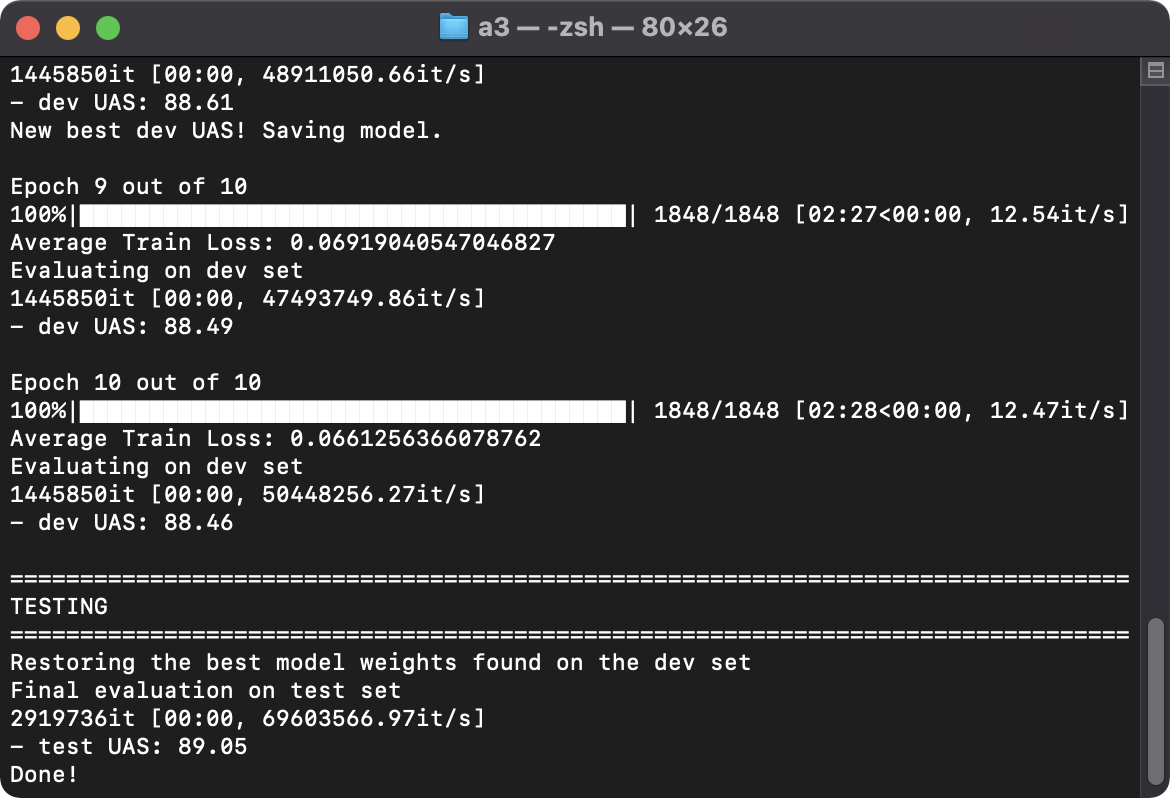
\includegraphics[width=0.5\textwidth]{best_uas.png}
            % \caption{test UAS after 10 epochs}
            \label{fig:parser result}
        \end{figure}

        dev UAS = 88.61, loss = 0.0661
        
        test UAS = 89.05

        \item 
        \begin{enumerate}[label=\roman*.]
            \item         
            \begin{itemize}
                % \item \textbf{Error type}: Verb Phrase Attachment Error                
                \item Error type: Verb Phrase Attachment Error
                \item Incorrect dependency: wedding $\rightarrow$ fearing
                \item Correct dependency: heading $\rightarrow$ fearing
            \end{itemize}

            \item
            \begin{itemize}
                \item Error type: Coordination Attachment Error
                \item Incorrect dependency: makes $\rightarrow$ rescue
                \item Correct dependency: rush $\rightarrow$ rescue
            \end{itemize}

            \item
            \begin{itemize}
                \item Error type: Prepositional Phrase Attachment Error
                \item Incorrect dependency: named $\rightarrow$ Midland
                \item Correct dependency: guy $\rightarrow$ Midland
            \end{itemize} 

            \item
            \begin{itemize}
                \item Error type: Modifier Attachment Error
                \item Incorrect dependency: elements $\rightarrow$ most
                \item Correct dependency: crucial $\rightarrow$ most
            \end{itemize} 
        \end{enumerate}   
        
    \end{enumerate}

\end{document} 